\section{神经机器翻译模型}
\label{sec:2_nmt}
在融合图片信息的神经机器翻译中,平行翻译句对的源语言句子与目标语言句子之间一般具有很强的语义对齐关系,而图片主要起到补充信息的作用。因此,ImgNMT所使用的模型多数是以神经机器翻译模型作为基础框架,视觉特征作为模型的额外输入。本节将介绍ImgNMT在模型设计发展过程中所应用到的神经机器翻译基础模型框架,这其中包含:基于循环神经网络(recurrent neural networks,RNN)方法的神经机器翻译(RNN-based neural machine translation,RNMT)模型\pcite{sutskever2014sequence,cho2014learning}、增加注意力机制的RNMT模型\pcite{bahdanau2015neural,luong2015effective}以及基于自注意力机制的Transformer\pcite{vaswani2017attention}。另外,还有基于卷积神经网络(convolutional neural networks,CNN)的NMT模型\pcite{gehring2017convolutional},但其很快被自注意力机制取代,也没有在ImgNMT任务上得到应用,因此本节忽略这部分内容的介绍。

\subsection{循环神经网络}
\label{sec:2_rnn}
\begin{figure}[!htbp]
    \centering
    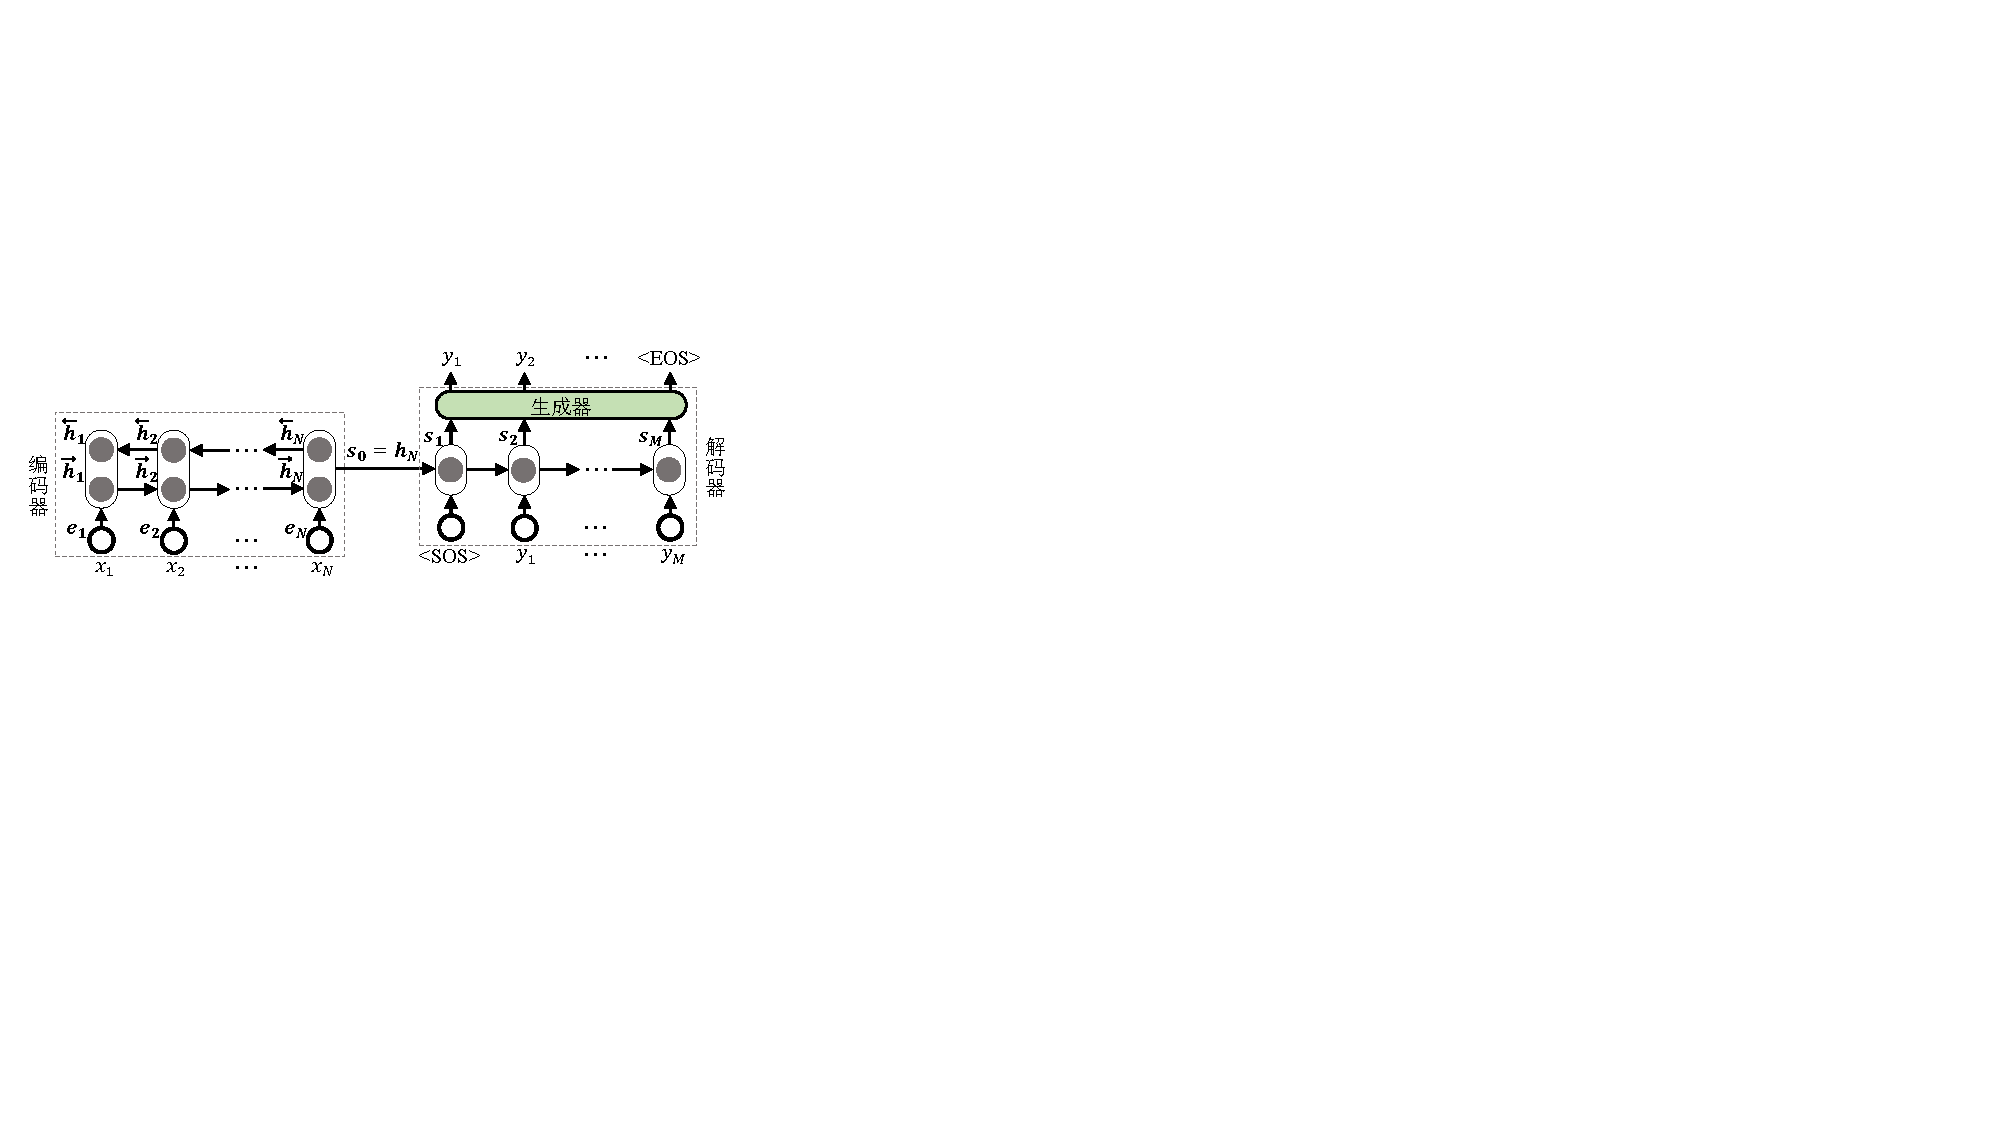
\includegraphics[scale=1]{Img/fig_2_rnmt.pdf}
    \bicaption{基于循环神经网络的神经机器翻译}{Neural machine translation based on recurrent neural network}
    \label{fig:2_rnmt}
\end{figure}
神经机器翻译是一种序列到序列的生成任务,其源端序列与目标端序列的长度往往是不同的。因此,编码器-解码器结构成为了神经机器翻译的常用模型框架。编码器和解码器分别用于编码源端序列和解码到目标端序列。循环神经网络就是一种用于解决序列建模问题的方法。图\ref{fig:2_rnmt}为基于循环神经网络的神经机器翻译框架。编码器将不定长的源语言句子编码为单个固定维度的隐层向量,该隐层向量可作为整个句子语义的特征表示。解码器负责根据该特征表示生成目标语言句子。形式化地,给定待翻译的源语言句子$X=\{x_1,x_2,…,x_N\}$,在编码端首先需要将$X$中的词转化为词向量$E=\{\Vector{e_1,e_2,…,e_n}\}$,其中:
\begin{equation}
    \Vector{e_i}=\mathrm{Emb}(x_i)
\end{equation}

源语言句子中的每个词$x_i$均有一个对应的词向量表示$\Vector{e_i}$。然后编码器按照句子中词的顺序将句子编码到一个隐层状态序列$\rarwvec{H}=\{\rarwvec{h}_1,\rarwvec{h}_2,…,\rarwvec{h}_N\}$,其中,$\rarwvec{h}_i$中编码了输入序列中前$i$项的信息,即:
\begin{equation}
    \rarwvec{h}_i=\mathrm{RNN}(\rarwvec{h}_{i-1},\rarwvec{e}_i)
\end{equation}
其中$\rarwvec{h}_{0}$可随机初始化或置为零向量。为了使每个位置的编码都能融合整个输入序列的信息,可采用双向编码器将句子$X$同时编码到$\rarwvec{H}$和$\larwvec{H}$,其中,$\larwvec{H}=\{\larwvec{h}_1,\larwvec{h}_2,…,\larwvec{h}_N\}$为$X$的逆序编码结果,即:
\begin{equation}
    \larwvec{h}_i=\mathrm{RNN}(\larwvec{h}_{i+1},\larwvec{e}_i)
\end{equation}
将$\rarwvec{H}$和$\larwvec{H}$拼接得到$\Vector{H=\{h_1,h_2,\cdots,h_N}\}$, 其中:
\begin{equation}
    \Vector{h_i}=[\rarwvec{h}_i;\larwvec{h}_i]
\end{equation}

RNMT的解码器同样采用循环神经网络生成目标语言文本。该生成翻译的过程是自回归的,即在时刻$t$,解码器需要根据$0$至$t-1$时刻的解码结果及源语言所提供的上下文信息进行当前时刻的预测结果的生成:
\begin{equation}
    \Vector{s}_t=\mathrm{RNN}(\Vector{s_{t-1}},y_{t-1})
\end{equation}
\begin{equation}
    P(y_t|y_{<t},X)=\mathrm{softmax}(g(\Vector{s_t}, y_{t-1}, \Vector{c_t}))
\end{equation}
该过程中,源端上下文信息的作用方式有很多种。\tcite{sutskever2014sequence}将$\rarwvec{h}_N$传递给解码器作为初始状态$\Vector{s_0}$。\tcite{cho2014learning}将$0$至$t-1$时刻的解码结果编码,并连同源端上下文信息$\Vector{H}$预测当前时刻单词:
\begin{equation}
    \Vector{c_t}=f(\Vector{H})
\end{equation}
其中,$f(\cdot)$表示选用平均池化(average pooling)对$\Vector{H}$取平均,或直接选取$\Vector{H}$的最后一项$\Vector{h_n}$。

虽然基于循环神经网络的神经机器翻译还没有实现对传统统计机器翻译在翻译准确率上的全面超越,但其采用的编码器-解码器框架已经展现了能够将文本数据进行分布式表示并从这种表示中解码到目标语言译文的能力。这种分布式表示方法也为跨模态信息的融合提供了极大的便利。

\subsection{注意力机制}
\label{sec:2_attention}
基于编码器-解码器结构的神经翻译模型利用编码器将源语言编码为一个固定的特征向量,再利用解码器中的循环神经网络编码已生成的目标端单词,从而指导新的目标端单词的生成。在该过程中,编码的源语言特征向量作为句子级语义的完整表示,一方面丢失了源语言中的句长信息,另一方面无法指导在当前时刻$t$生成目标端单词时应该更多地关注源端的哪些信息。为了解决这个问题,\tcite{bahdanau2015neural}提出在编码器与解码器之间增加注意力机制(attention mechanism)。

\begin{figure}[!htbp]
    \centering
    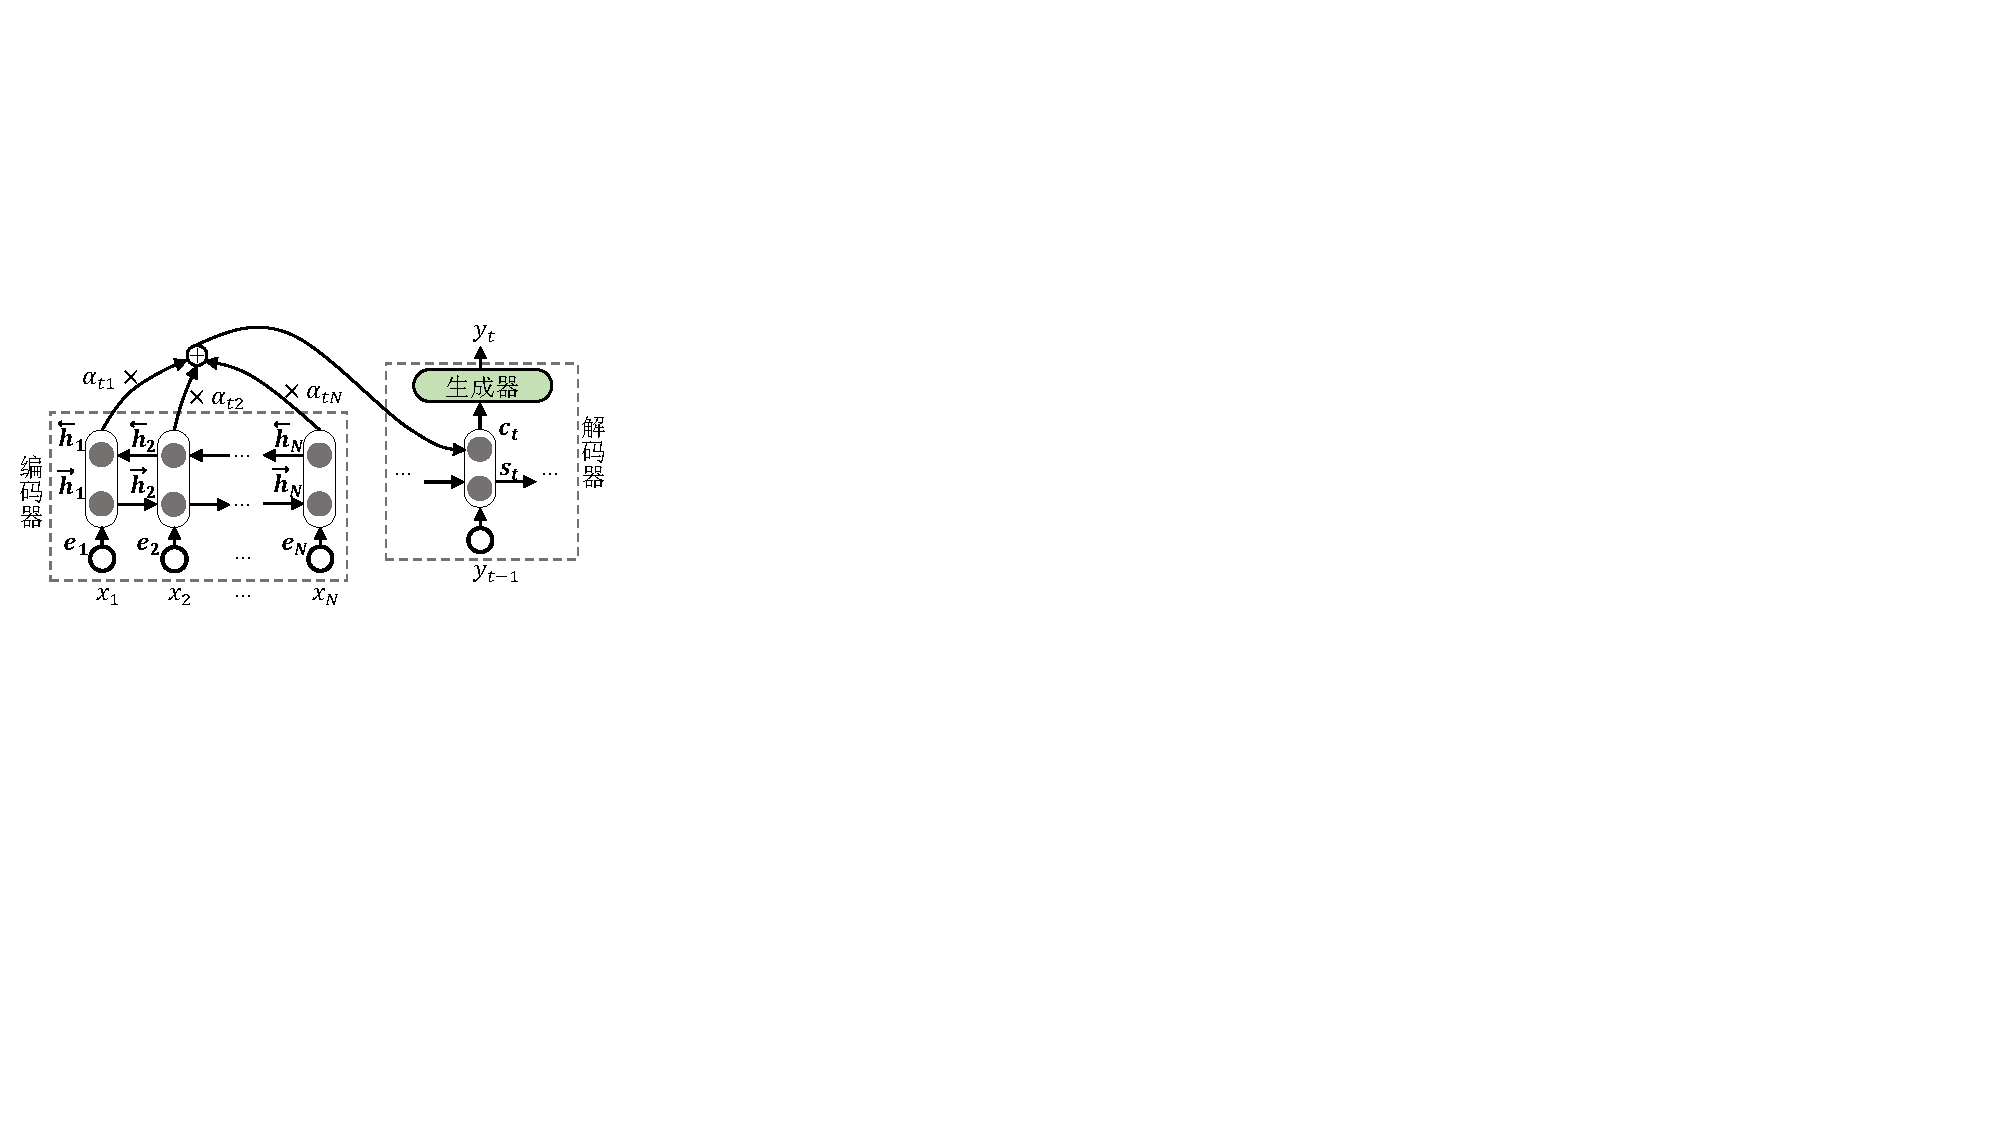
\includegraphics[scale=1]{Img/fig_2_att_rnmt.pdf}
    \bicaption{增加注意力机制的RNMT}{Attention-based RNMT}
    \label{fig:2_att_rnmt}
\end{figure}
图\ref{fig:2_att_rnmt}为增加了注意力机制的神经机器翻译,其编码器和解码器保留原来的工作方式,而两者之间的注意力模块为解码器提供了动态的源语言上下文信息。对于每个时刻$t$,源语言上下文向量$\Vector{c_t}$由固定的特征向量替换为与$t$相关的表示:
\begin{equation}
    \Vector{c_t} = f_t(\Vector{H})=\sum_{i=1}^{N}{\alpha}_{ti}\Vector{h_i}
\end{equation}
\begin{equation}
    {\alpha}_{ti}=\frac{\mathrm{exp}(a_{ti})}{\sum_{j=1}^{n}\mathrm{exp}(a_{tj})}
\end{equation}
\tcite{bahdanau2015neural}所提方法中:
\begin{equation}
    a_{ti} = \mathrm{score}(\Vector{s_{t-1},h_i})
\end{equation}
其中$\mathrm{score}(\cdot)$是打分函数,计算两个向量所携带信息的相关程度,可采用点积或多层感知机等方法。上式对$\Vector{s_{t-1}}$和$\Vector{h_i}$进行打分,表示根据已生成的目标文本编码表示$\Vector{s_{t-1}}$,计算源语言中第$i$项对当前时刻$t$的重要程度。因此,$a_{ti}$代表着生成$t$时刻的目标端单词时,对源语言中第$i$项的“关注”度,${\alpha}_{ti}$就是该“关注”度的归一化结果,$\Vector{c_t}$就是根据“关注”度对特征向量的加权表示。

值得注意的是,$t-1$时刻的输出结果$y_{t-1}$是由$\Vector{s_{t-1}}$得到的,因此上式中丢失了$y_{t-1}$的信息,\tcite{luong2015effective}提出了改进方案:
\begin{equation}
    a_{ti} = \mathrm{score}(\Vector{s_{t},h_i})
\end{equation}
并规定了$\mathrm{score}(\cdot)$的三种计算方式,综合\tcite{bahdanau2015neural}等提出的方法,可得到以下四种方法:
\begin{equation}
    \mathrm{score}(\Vector{s_t, h_i}) = 
    \begin{cases}
        \Vector{s_t^T h_i} & \mbox{{\itshape 点积法}} \\
        \Vector{s_t^T W_a h_i} & \mbox{{\itshape 通用点积法}} \\
        \Vector{W_a[s_t; h_i]} & \mbox{{\itshape 连接法}} \\
        \Vector{v_a^T} \mathrm{tanh}(\Vector{W_a s_t+U_a h_i}) & \mbox{{\itshape 多层感知机法}} 
    \end{cases}
\end{equation}
其中$\Vector{v_a}$、$\Vector{W_a}$和$\Vector{U_a}$是网络参数,$T$表示对向量进行转置。

%(注意力机制在视觉领域的应用,以及在跨模态领域的应用。)

\subsection{Transformer}
\label{sec:2_transformer}
\begin{figure}[!htbp]
    \centering
    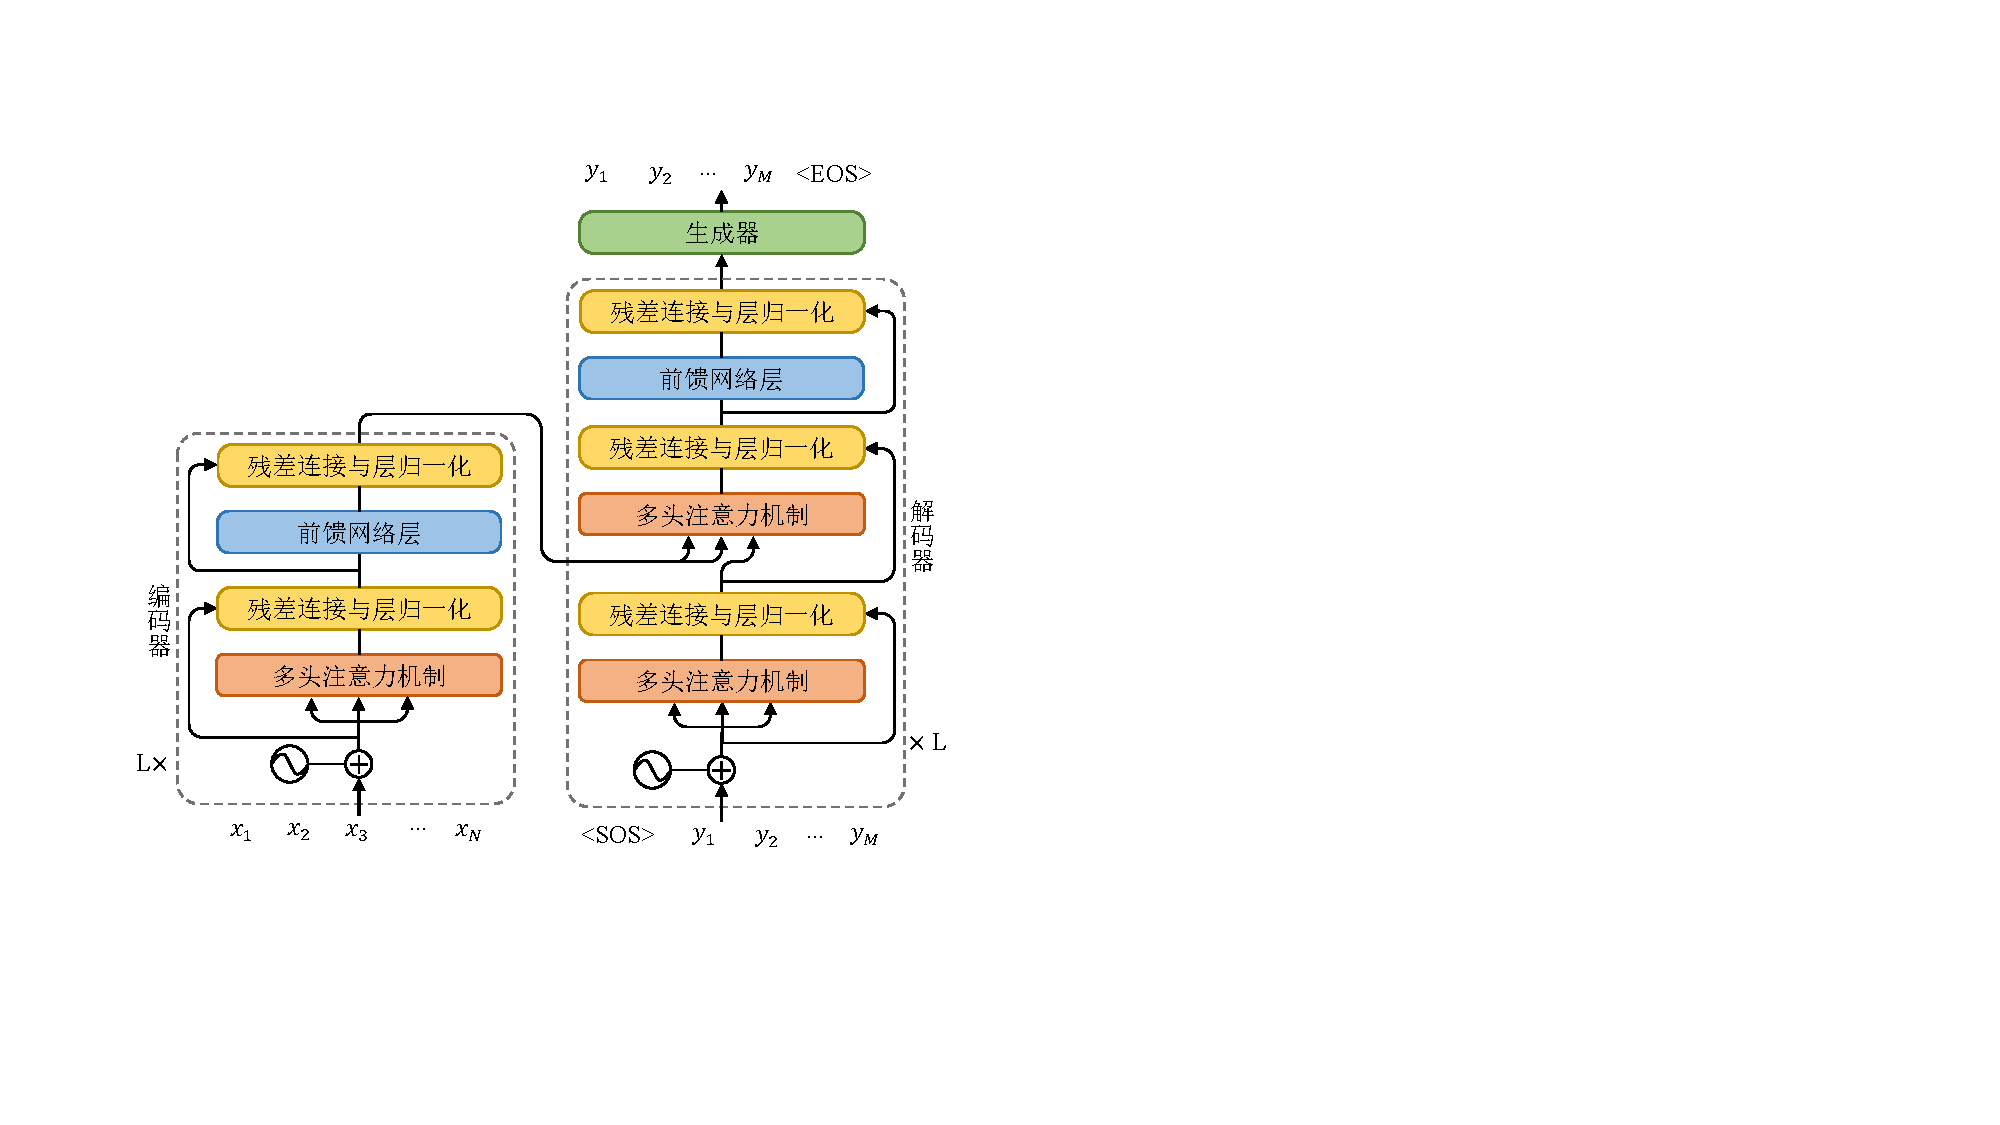
\includegraphics[scale=1]{Img/fig_2_transformer.pdf}
    \bicaption{基于Transformer的神经机器翻译}{Transformer-based neural machine translation}
    \label{fig:2_transformer}
\end{figure}
在注意力机制的帮助下,基于循环神经网络的神经机器翻译得到了显著的性能提升。这说明基于动态上下文的解码方法能够更准确地捕捉上下文信息,从而得到更忠于原文的译文。而注意力机制相当于二次编码,为下游模块提供动态上下文。既然注意力机制同样具有编码能力,那么是否可以用于替换循环神经网络呢?谷歌提出的Transformer\pcite{vaswani2017attention}就是一种基于这种假设的模型。图\ref{fig:2_transformer}展示了Transformer的模型结构,其保留了编码器-解码器的基础框架,利用内置的多头注意力机制(multi-head attention mechanism)实现编码与解码过程。


\begin{figure}[!htbp]
    \centering
    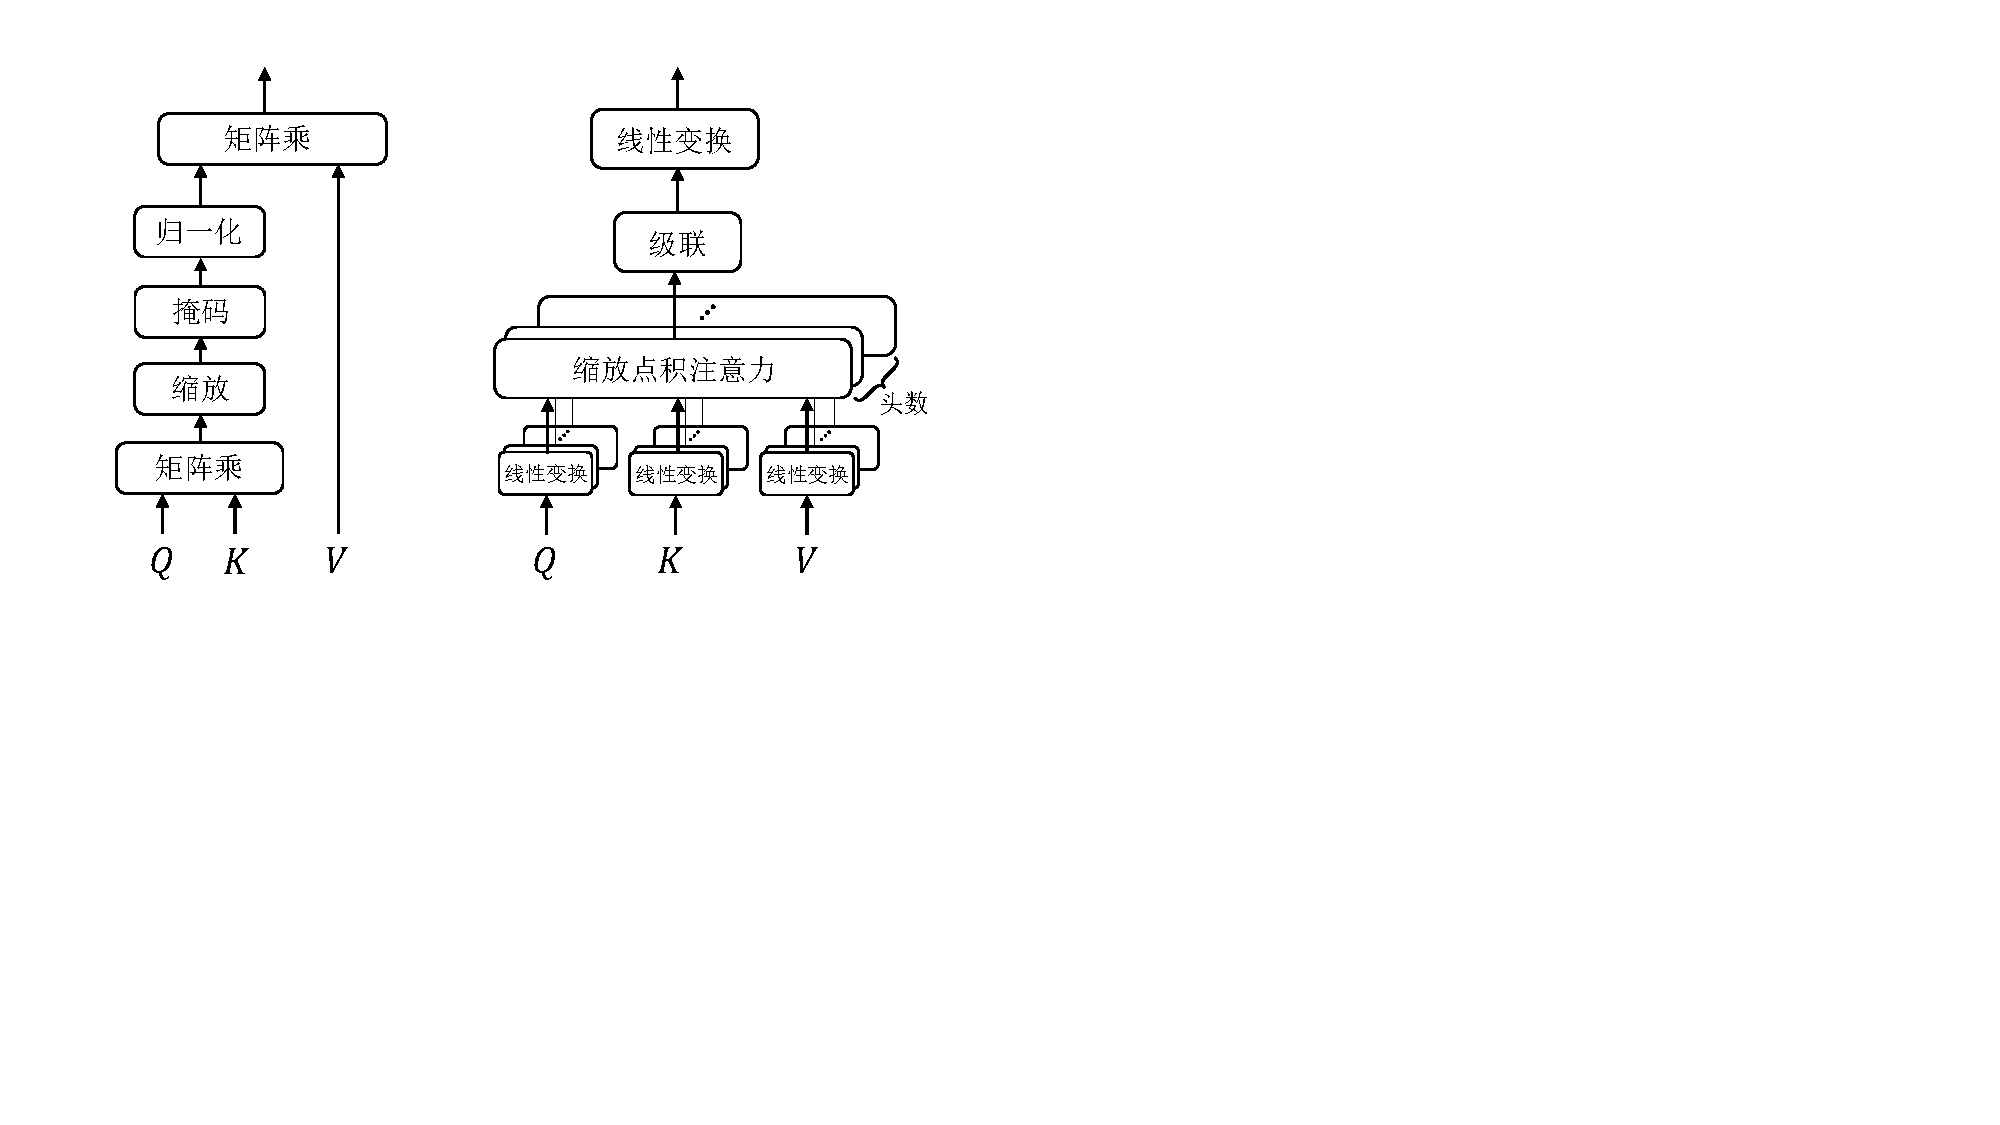
\includegraphics[scale=0.8]{Img/fig_2_multihead.pdf}
    \bicaption{多头注意力机制框架图}{Frame diagram of multi-head attention mechanism}
    \label{fig:2_multihead}
\end{figure}
区别于一般的注意力机制,多头注意力机制采用了一种更具泛化性的模型设计。如图\ref{fig:2_multihead}所示,多头注意力机制的输入分为查询(query,Q)、键(key,K)以及值(value,V)三部分,并结合了缩放点积注意力(scaled dot-product attention)和多头注意力(multi-head attention)两种方法。

{\sffamily 缩放点积注意力:}与一般的点积法相比,缩放点积注意力增加了一个缩放因子$d_k^{-0.5}$:
\begin{equation}
    \mathrm{Attention}(\Vector{Q},\Vector{K},\Vector{V}) = \mathrm{softmax} \left( \frac{\Vector{Q}\Vector{K}^T}{\sqrt{d_k}} \right) \Vector{V}
\end{equation}
其中,$d_k$代表$\Vector{Q}$、$\Vector{K}$和$\Vector{V}$的隐层维度。采用点积法的优点在于点积是以矩阵乘的形式进行计算,通过底层代码优化等方法可以很好地对矩阵乘进行硬件加速。引入缩放因子则是为了防止$d_k$较大时,点积的数值膨胀导致$\mathrm{softmax}(\cdot)$函数逼近梯度消失的数值范围。

{\sffamily 多头注意力:}为了丰富动态上下文所承载的信息,\tcite{vaswani2017attention}将多个注意力模块拼接组成多头注意力机制:
\begin{equation}
    \mathrm{MultiHead}(\Vector{Q,K,V}) = \mathrm{Concat}(\Vector{head_1, \cdots, head_n})\Vector{W^O}
\end{equation}
\begin{equation}
    \Vector{head_i} = \mathrm{Attention}(\Vector{Q W_i^Q,K W_i^K,V W_i^V})
\end{equation}
其中,$\Vector{W^O}$,$\Vector{W_i^Q}$,$\Vector{W_i^K}$和$\Vector{W_i^V}$是模型参数。$\Vector{Q}$、$\Vector{K}$和$\Vector{V}$经过不同的参数映射到不同的表示空间,再由注意力机制编码得到的不同的上下文特征表示。该过程相当于在不增加额外参数的情况下,将多个模型集成到一个模型中,从而提升模型的学习能力。

多头注意力机制在Transformer中的用途分为三种:
\begin{itemize}
    \item 位于编码器的多头自注意力机制用于编码源语言句子,此时Transformer编码器第一层的$\Vector{Q}$、$\Vector{K}$和$\Vector{V}$均为源语言句子经映射后的词向量序列,其它层的$\Vector{Q}$、$\Vector{K}$和$\Vector{V}$为前一层的输出。
    \item 位于解码器中带有掩码的多头自注意力机制用于编码目标端已经解码出来的部分句子。掩码的作用是为了保持自回归解码过程中后面位置单词的解码只能用到前面位置信息的特性。
    \item 连接编码器与解码器的多头交叉注意力机制的作用和一般的注意力机制相似。此时$\Vector{Q}$为解码器中带有掩码的多头自注意力机制的输出,$\Vector{K}$和$\Vector{V}$为编码器的隐层输出。交叉注意力机制输出的是融合了源端信息的目标端句子的表示。
\end{itemize}

值得注意的是,基于多头自注意力机制的编码过程与循环神经网络相比丢失了对输入序列位置信息的建模。因此,\tcite{vaswani2017attention}提出了位置编码(positional encoding),为每个词向量增加位置信息。%文献\cite{DBLP:journals/corr/GehringAGYD17}则提出了更为方便的位置词向量的方案。

尽管近年来针对Transformer框架的改动层出不穷,但广泛应用的模型基本保持了最原始的设计方案。常见的改动如\tcite{devlin2019bert}提出了使用位置词向量(positional embedding)的方式替换位置编码,以及为了加强Transformer对长序列的编码能力提出相对位置编码\pcite{shaw2018self,dai2019transformerxl}。而这些创新性的改动基本都保留了Transformer中的自注意力机制和交叉注意力机制的基本结构。除了机器翻译等生成式任务外,在大规模预训练任务的表现上,Transformer更是充分展现了其应用场景的灵活性\citep{radfordimproving,devlin2019bert,liu2019roberta,lewis2020bart,raffel2020exploring}。针对不同规模的数据,通过增减参数规模的方式就可以使其适应相应的任务。相比于基于循环神经网络的模型,Transformer能够容纳更长的输入序列和更大规模的网络参数。

Transformer出色的编码能力不仅在自然语言处理任务大放异彩,还在计算机视觉以及多模态信息融合等领域展现了不俗的潜能。例如在计算机视觉领域的图像分类、目标检测以及语义分割等传统任务上摒弃了基于卷积神经网络的方法,直接采用Transformer作为基础模型,并在多个任务上得到了进一步的性能提升\pcite{parmar2018image,dosovitskiy2021vit,liu2021swin,yuan2021tokens};或是在大规模文本预训练模型的基础上,在输入序列中增加图片输入或从图片中提取的视觉目标,提升Transformer在多模态自然语言理解(multi-modal natural language understanding)任务上的能力\pcite{lu2019vilbert,chen2020uniter,huang2020pixelbert,kim2021vilt}。

%(Transformer已经在业界产生的影响力,自注意力替换循环神经网络的必要性,解决了哪些问题)
